\documentclass[11pt]{article}
\usepackage[margin=1.1in]{geometry}
\usepackage{my_symbols}
\usepackage{hyperref}
\newcommand{\MEKA}{Meka}
\newcommand{\MICE}{Mice}
\newcommand{\MOA}{Moa}
\newcommand{\WEKA}{Weka}
\newcommand{\MULAN}{Mulan}
\def\version{{\tt 2.0.0}}
\usepackage{listings}

\definecolor{mygreen}{rgb}{0,0.6,0}
\definecolor{mygray}{rgb}{0.5,0.5,0.5}
\definecolor{mymauve}{rgb}{0.58,0,0.82}

\usepackage{courier}
\lstset{
	tabsize=2,
	backgroundcolor=\color{white},   % choose the background color
	breaklines=true,                 % automatic line breaking only at whitespace
	captionpos=b,                    % sets the caption-position to bottom
	commentstyle=\color{mygreen},    % comment style
	escapeinside={\%*}{*)},          % if you want to add LaTeX within your code
	keywordstyle=\color{blue},       % keyword style
	stringstyle=\color{mymauve},     % string literal style
	basicstyle=\footnotesize,        % size of fonts used for the code
	basicstyle=\small\ttfamily,
	breaklines=true,
	xleftmargin=\parindent
}
%\lstset{framextopmargin=50pt,frame=bottomline}
%\lstset{breaklines=true} 
%\lstset{breakatwhitespace=true} 

% if you just need a simple heading
% Usage:
%   \heading{the text of the heading}
\newcommand{\heading}[1]{
    \vspace{0.3cm} \noindent \textbf{#1} \newline
}

\usepackage{datetime}
\newdateformat{mydate}{\monthname[\THEMONTH] \THEYEAR}

\begin{document}

\title{Tutorial. \framework{\MEKA} \version }

%\author{The \framework{\MEKA} Team}

\date{\mydate\today}

\maketitle

\begin{center}
	
\includegraphics{MEKA.png}\\
		A Multilabel/multitarget Extension to WEKA.\\
		\url{http://meka.sourceforge.net}
\end{center}

\tableofcontents

\thispagestyle{empty}
\pagebreak

\section{Introduction}

This is a tutorial for the open source machine learning framework \framework{\MEKA}. \framework{\MEKA} is closely based upon the \framework{\WEKA} framework \cite{WEKA}; providing support for development, running and evaluation of \keyword{multi-label} and \keyword{multi-target} classifiers (which \framework{WEKA} does not).

In the \keyword{multi-label} problem, a data instance may be associated with multiple labels. This is as opposed to the traditional task of single-label classification (\ie multi-class, or binary) where each instance is only associated with a single class label. The multi-label context is receiving increased attention and is applicable to a wide variety of domains, including text, music, images and video, and bioinformatics. A good introduction can be found in \cite{MMD} and \cite{Thesis}.

The multi-label problem is in fact a special case of \keyword{multi-target} learning. In multi-target, or \textit{multi-dimensional} learning, a data instance is associated with multiple target variables, where each variable takes a number of values. In the multi-label case, all variables are binary, indicating label relevance ($1$) or irrelevance ($0$). The multi-target case has been investigated by, for example, \cite{UPM} and \cite{MT}.  

\framework{\MEKA} can also includes \emph{incremental} classifiers suitable for the \keyword{data streams} context. An overview of some of the methods included in \framework{\MEKA} for learning from incremental data streams is given in \cite{MEDS2}.

\framework{\MEKA} is released under the GNU GPL v3 licence. The latest release, source code, API reference, this tutorial, and further information and links to additional material, can be found at the website: \url{http://meka.sourceforge.net}. 

This tutorial applies to \framework{\MEKA} version {\version}. 

\section{Getting Started}

\framework{\MEKA} can be download from: \url{http://sourceforge.net/projects/meka/files/}. This tutorial is written for version \version; and assumes that you have downloaded and extracted {\green the \texttt{meka-release-\version} and that \texttt{meka-\version}, found within, is your current working directory.
}

\subsection{Requirements}

\framework{\MEKA} requires:

\begin{itemize}
	 \item Java version 1.6 or above
\end{itemize}

%\subsection{Downloading}
{\green
\framework{\MEKA} comes bundled with other packages such as \framework{\WEKA}'s \texttt{weka.jar}, and also \framework{\MULAN}'s \texttt{mulan.jar} for running classifiers from this framework. % If \framework{\WEKA} is already installed on your system, it must be at least version release (\texttt{3.7.X}) to be compatible with \texttt{\MEKA}.
These files are found in the \texttt{lib} directory. See \texttt{lib/README.txt} for version information.
}


%\framework{\MEKA}'s incremental classification extension (\texttt{mice.jar}) comes packaged in a separate jar file. 

\subsection{Running}
\label{sec:running}

\framework{\MEKA} can be used very easily from the command line. For example, to run the Binary Relevance (BR) classifier on the \textit{Music} dataset; {\green type:
\begin{lstlisting}
java -cp "./lib/*" meka.classifiers.multilabel.BR -t data/Music.arff
\end{lstlisting}
}

If you are on a Microsoft Windows system, you need to use back slashes instead of forward slashes (\texttt{.\textbackslash lib\textbackslash*}). If you add the \texttt{jar} files to the system's \texttt{CLASSPATH}, you do not need to supply the \texttt{-cp} option at runtime. For the remainder of examples in this tutorial we will assume that this is the case.

Since Version 1.2 \framework{\MEKA} has a graphical user interface (GUI). Run this with either the \texttt{run.sh} script (under Linux or OSX) as follows:
\begin{lstlisting}
./run.sh
\end{lstlisting}
Run \texttt{run.bat} instead if you are using Microsoft windows.


%\begin{lstlisting}
%	export CLASSPATH=$MEKA/meka.jar:$MEKA/weka.jar:$CLASSPATH
%\end{lstlisting}
%
%where \texttt{\$MEKA} is the folder you extracted the software to; or by supplying the classpath directly when running java with :


\section{\label{sec:format}\framework{\MEKA}'s Dataset Format}

\framework{\MEKA} uses \framework{\WEKA}'s ARFF file format. See \url{http://weka.wikispaces.com/ARFF} to learn about this format. \framework{\MEKA} uses multiple attributes -- one for each target or label -- rather than a single class attribute. The \emph{number} of target attributes is specified with either \texttt{-C} or \texttt{-c}; \emph{unlike} in \framework{\WEKA} where the \texttt{-c} flag indicates the position of the \emph{class index}. \framework{\MEKA} uses the reference to the \texttt{classIndex} internally to denote the number of target attributes. %This is important when creating new \framework{\MEKA} classifiers (see Section \ref{sec:extending}).

Since the number of target attributes tends to vary with each dataset, for convenience \framework{\MEKA} allows this option (as well as other dataset options like the train/test split percentage) to be stored in the \texttt{@relation} name of an ARFF file, where a colon (\texttt{:}) is used to separate the dataset name and the options. The following is an example ARFF header for multi-target classification with three target variables and four attributes:
 
{\small

\begin{lstlisting}
@relation 'Example_Dataset: -C 3'

@attribute category {A,B,C,NEG}
@attribute label {0,1}
@attribute rank {1,2,3}
@attribute X1 {0,1}
@attribute X2 {0,1}
@attribute X3 numeric
@attribute X4 numeric

@data
\end{lstlisting}
}

Note that the format of the \texttt{label} attribute (binary) is the \emph{only} kind of target attribute in multi-\emph{label} datasets. For more examples of \framework{\MEKA} ARFF files; see the \texttt{data/} directory for several multi-label and multi-target datasets (some of these are in a compressed format).

\framework{\MEKA} can also read ARFF files in the \framework{\MULAN} format where target attributes are the \emph{last} attributes, rather than the first ones. This format can also be read by \framework{\MEKA} by specifying a minus sign `\texttt{-}' before the number of target attributes in the \texttt{-C} option. For example, \texttt{-C -3} will set the \emph{last} \texttt{3} attributes as the target attributes automatically when the file is loaded. Alternatively, the target attributes can be moved using \framework{\WEKA}'s \texttt{Reorder} filter, or in the GUI as detailed in the following section. %weka.filters.unsupervised.attribute.

%Note that the \framework{\MULAN} format expects the target attributes to be indexed \emph{last} rather than the first. Specifying \texttt{-c $-L$} to \framework{\MEKA} will automatically move the last $L$ attributes to the beginning upon loading. 

\subsection{Manipulating Datasets in the GUI}
\label{sec:data.gui}

A good way to set up an ARFF file for multi-dimensional classification is using the GUI. Open an ARFF file with `\textsf{Open}' from the \textsf{File} menu. In the \textsf{Preprocess} tab in the right-hand column (see \Fig{screen:arff}; note that the class attributes are listed in \textbf{bold} face), simply select the attributes you wish to use as class attributes and click the button `\textsf{Use class attributes}'. You can then save this file using `\textsf{Save}' from the \textsf{File} menu, which will also save the \texttt{-C} flag into the \texttt{@relation} tag as described above (displayed under '\textsf{Relation:}' in the GUI), so next time the classes will be set automatically.

The datasets that come with \framework{\MEKA} already come with the \texttt{-C} flag specified correctly, so you do not need to set this information.

You can also run any of \framework{\WEKA}'s filters on the dataset with the \textsf{Choose} button. See the \framework{\WEKA} documentation for more information.

\begin{figure}
	\centering
	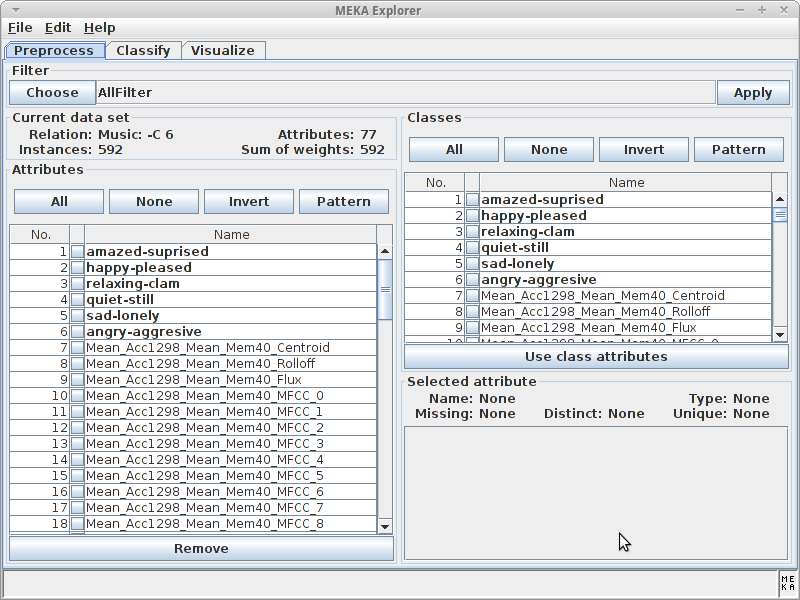
\includegraphics[height=0.75\textwidth]{GUI01.png}
	\caption{\label{screen:arff} \framework{MEKA}'s GUI interface; having loaded the \textit{Music} dataset.}
\end{figure}

\section{Using \framework{\MEKA}}%: Running Experiments

%With any suitable dataset it is possible t\framework{\MEKA} classifiers.
A suitable dataset is the only requirement to begin running experiments with \framework{\MEKA}.

\subsection{Command Line Interface}

With the exception of the different use of the \texttt{-c} flag (see the previous section), many of \framework{\WEKA}'s command line options for evaluation work identically in \framework{\MEKA} too. You can obtain a list of them by running any classifier with the \texttt{-h} flag, for example running \texttt{java meka.classifiers.multilabel.BR -h} on the command line results in the output:
	 
\begin{center}
\lstinputlisting[basicstyle=\scriptsize\ttfamily,frame=single,firstline=2,lastline=56]{help.txt}
\end{center}

Note that the only required option is just \texttt{-t} to specify the dataset (and \texttt{-C} to specify the number of target attributes, if not already included within the dataset \texttt{@relation} tag, as explained in the previous section). Note also that the \texttt{Classifier Options} are specific to each classifier (which in this case is \texttt{BR}), and each base classifier (for \texttt{BR}, the default base classifier is \texttt{J48}). The \texttt{J48}-specific options (which are truncated in this output) are visible following the hyphen (\texttt{-}). 

\texttt{BR} has limited options, for example to change the base classifier (the \texttt{-W} option). For example, to use Naive Bayes, type\footnote{If typed on one line, the backslash `\texttt{\textbackslash}' should be omitted} on the command line:

\begin{lstlisting}
java meka.classifiers.multilabel.BR -t data/Music.arff \
  -W weka.classifiers.bayes.NaiveBayes
\end{lstlisting}

\subsection{Graphical User Interface}

The CLI is the most powerful way to work with \framework{\MEKA}, but the GUI is a good way to get started. Refer to \Sec{sec:running} on how to open the GUI. Once opened, you will see three tabs: \textsf{Preprocess}, \textsf{Classify}, \textsf{Visualize}. The following process will guide you through a simple experiment.


\begin{enumerate}
	\item Load a dataset file using \textsf{Open} from the file menu. %See \Sec{sec:data.gui} for information on preprocessing the datasets.
	\item Click on the \textsf{Classify} tab.
	\item \textsf{Choose} a multi-label or multi-target classifier (or leave the default choice). 
	\item Click on the label to the right of this button and set specific options to the classifier. In most cases, these options also involve setting a \framework{\WEKA} single-label base classifier (and also its options). For \framework{\MEKA}'s \texttt{meta} classifiers, you will need to first choose a multi-label base classifier, and then a single-label (\framework{\WEKA}) base classifier for this classifier. See, for example, \Fig{screen:eval}, using a \texttt{BaggingML} ensemble of \texttt{CC} (classifier chains) with \texttt{SMO} as the single-label base classifier.
	\item In the \textsf{Evaluation} panel you configure what type of evaluation you want to do, and some of the options given in the previous section are available here. For example, a 55/45 train/test split, as being specified in \Fig{screen:split}.
	\item When you click \textsf{Start} the experiment will be run. When finished, the result will appear in the \textsf{History} panel. This is the same output as would be seen on the command line, and explained in the following section. The verbosity of the results is controlled by the \textsf{Verbosity} option.
	%\item You can export results to text, or copy of paste it.
	\item (Optional) View the Precision-Recall curves by right-clicking on the results and selecting \textsf{Show Precision-Recall}.
	\item (Optional) If you chose a \texttt{MultiLabelDrawable} classifier (such as \texttt{BR}, \texttt{CC}, \texttt{LP}, or any derivatives) and a \texttt{Drawable} base classifier such as \texttt{J48}, you can right click on the results and select \textsf{Show Graphs}.
	\item (Optional) Click on the \textsf{Visualize} tab inspect the dataset.
\end{enumerate}




\begin{figure}
	\centering
	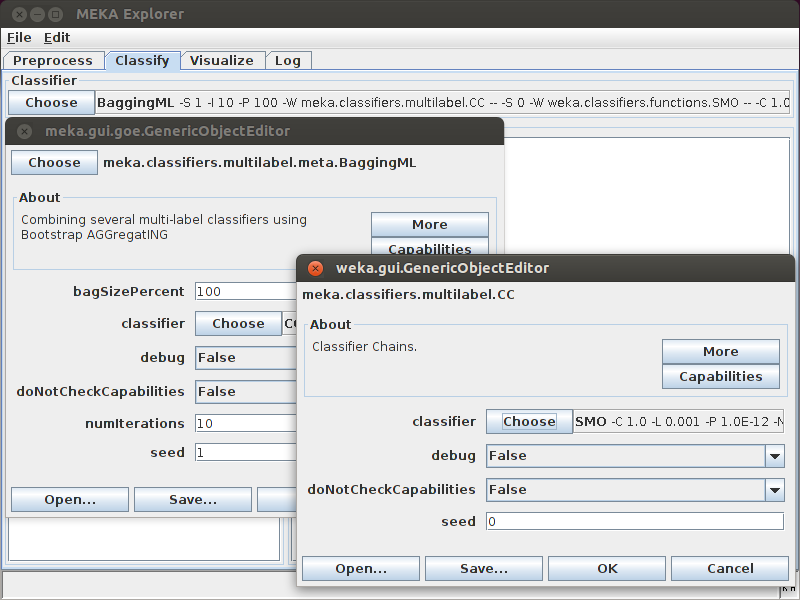
\includegraphics[height=0.60\textwidth]{GUI02.png}
	\caption{\label{screen:eval} \framework{MEKA}'s GUI interface; setting Bagging of Classifier Chains with SMO.}
\end{figure}


\begin{figure}
	\centering
	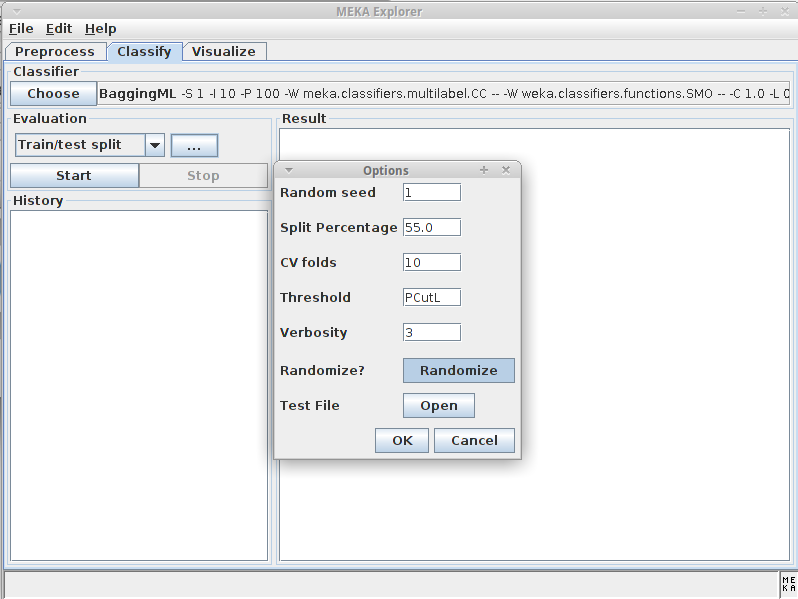
\includegraphics[height=0.60\textwidth]{GUI03.png}
	\caption{\label{screen:split} \framework{MEKA}'s GUI interface; setting a train/test split.}
\end{figure}

\subsection{\label{sec:evaluation}Evaluation}

Running \texttt{BR} {\green with \texttt{NaiveBayes}} on the \textit{Music} data will output the following:

%\lstinputlisting{eval.txt}
\begin{center}
%\lstinputlisting[basicstyle=\scriptsize\ttfamily,frame=single]{../../../test/resources/meka/classifiers/%multilabel/BR.ref}
\lstinputlisting[basicstyle=\scriptsize\ttfamily,frame=single]{eval.txt}
\end{center}

\begin{figure}
	\centering
	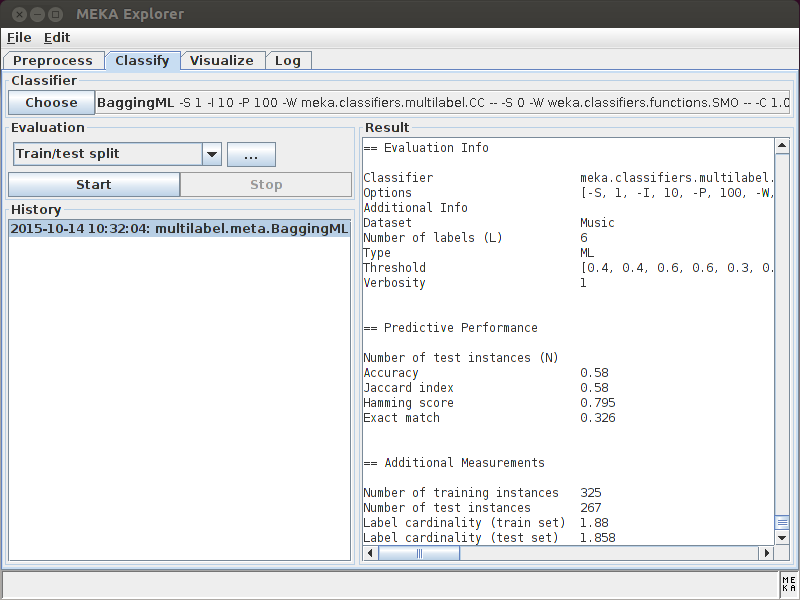
\includegraphics[height=0.95\textwidth]{GUI04.png}
	\caption{\label{screen:result} \framework{MEKA}'s GUI interface; results.}
\end{figure}

The results of the experiment in \Fig{screen:split} are shown in \Fig{screen:result}. Note that by increasing the verbosity level, you can get more or less output. On the command line, this is with \texttt{-verbosity <n>} where \texttt{<n>} = 
\begin{center}
\begin{tabular}{ll}
	\hline
	\texttt{verbosity}       & Output \\
	\hline
	\texttt{1} (default) & basic output \\
	 \texttt{2}           & plus more metrics \\
	  \texttt{3}           & plus individual metrics (for each label) \\
	   \texttt{4}           & plus more individual metrics (for each label) \\
		\texttt{5}           & plus individual classifications \\
	  \texttt{6}           & plus individual confidence outputs (rounded to 1 d.p.) \\
	   \texttt{7}           & \ldots (rounded to 2 d.p.) \\
		\texttt{8}           & \ldots (rounded to 3 d.p.) \\
	\hline
\end{tabular}
\end{center}
Note that some measures may be computationally intensive to calculate! Low verbosity levels will lead to faster evaluation times.

Most of these metrics are described in \cite{ECC2,MMD}. The most common metrics reported in the multi-label literature are \texttt{Hamming Loss} (evaluation by label, averaged across all labels) and \texttt{Exact Match} (evaluation of each example, averaged across all examples). Multi-label \texttt{Accuracy} (also called \texttt{Jaccard Index} in information retrieval) is a good compromise between both these metrics.

%\subsection{Thresholds}

Note that a \texttt{Threshold} can be calibrated automatically whenever \texttt{-threshold PCut}, by minimizing the difference between the label cardinality of the training set and the predictions on the test set\footnote{This does \emph{not} require access to the true predictions in the test set} \cite{ECC2}, the so-called \textit{P-Cut} method. To calibrate a threshold the same way but for each label individual, use instead \texttt{-threshold PCutL} option. This is being specified in \Fig{screen:split}, (note that one threshold is calibrated for each label in \Fig{screen:result}. In \textsf{Prequential} evaluation, only a fixed threshold is allowed.

%\begin{lstlisting}
%          Threshold : [0.29971988795518206, 0.26330532212885155, \
%			  0.4257703081232493, 0.22128851540616246, 0.23809523809523808, \
%			  0.3473389355742297]
%\end{lstlisting}

\framework{\MEKA} also supports \textsf{Cross-validation}; for example:
\begin{lstlisting}
java meka.classifiers.multilabel.BR -x 10 -R -t data/Music.arff \
  -W weka.classifiers.bayes.NaiveBayes
\end{lstlisting}
conducts 10 fold cross validation on a randomised version of the \textit{Music} dataset and outputs the average results across all folds with standard deviation. Note that under incremental evaluation, the \texttt{-x} option is reused to indicate the number of samples to take. %Note that using the \texttt{-f} option in this case to save output to a file will output only the results of the validation; which can be useful for compiling results later.

%Sometimes it can be useful to analyse the actual predictions made at test time (for example if you wish to use an evaluation metric not included in \framework{\MEKA}). \framework{\MEKA} can produce plain-text files with the option \texttt{-f <file name>}; for example:
%\begin{lstlisting}
%java meka.classifiers.multilabel.BR -t data/Music.arff \ 
%  -f BR-NB.meka \
%  -W weka.classifiers.bayes.NaiveBayes
%\end{lstlisting}
%which produces the plain-text file \texttt{BR-NB.meka}. This provides a way to do further evaluation `offline'. Note that when cross validation (\texttt{-x}) is used, %one file will be created for each fold, e.g., \texttt{BR-NB.meka.0}, \ldots, \texttt{BR-NB.meka.4} for a 5-fold validation. The results can be recalculated for any of %these files with, e.g.:
%\begin{lstlisting}
%	java weka.core.Result -f BR-NB.meka
%\end{lstlisting}
%Or, if you used cross validation, with:
%\begin{lstlisting}
%	java weka.core.Result -f BR-NB.meka -x 5
%\end{lstlisting}
%In this way, it is also possible to use \framework{\MEKA}'s evaluation procedures with output from other software (simply by using the right text output format).

If the multi-label classifier implements \texttt{MultiLabelDrawable} (such as \texttt{BR}, \texttt{CC}, \texttt{LP}, and classifiers which \texttt{extend} these) and if the base classifier implements \texttt{Drawable} (such as \texttt{J48}), you can right click on the results in the \textsf{History} tab and select \textsf{Show Graphs} and \textsf{Save Graphs}. This is exemplified in \Fig{screen:graphs}.

\begin{figure}
	\centering
	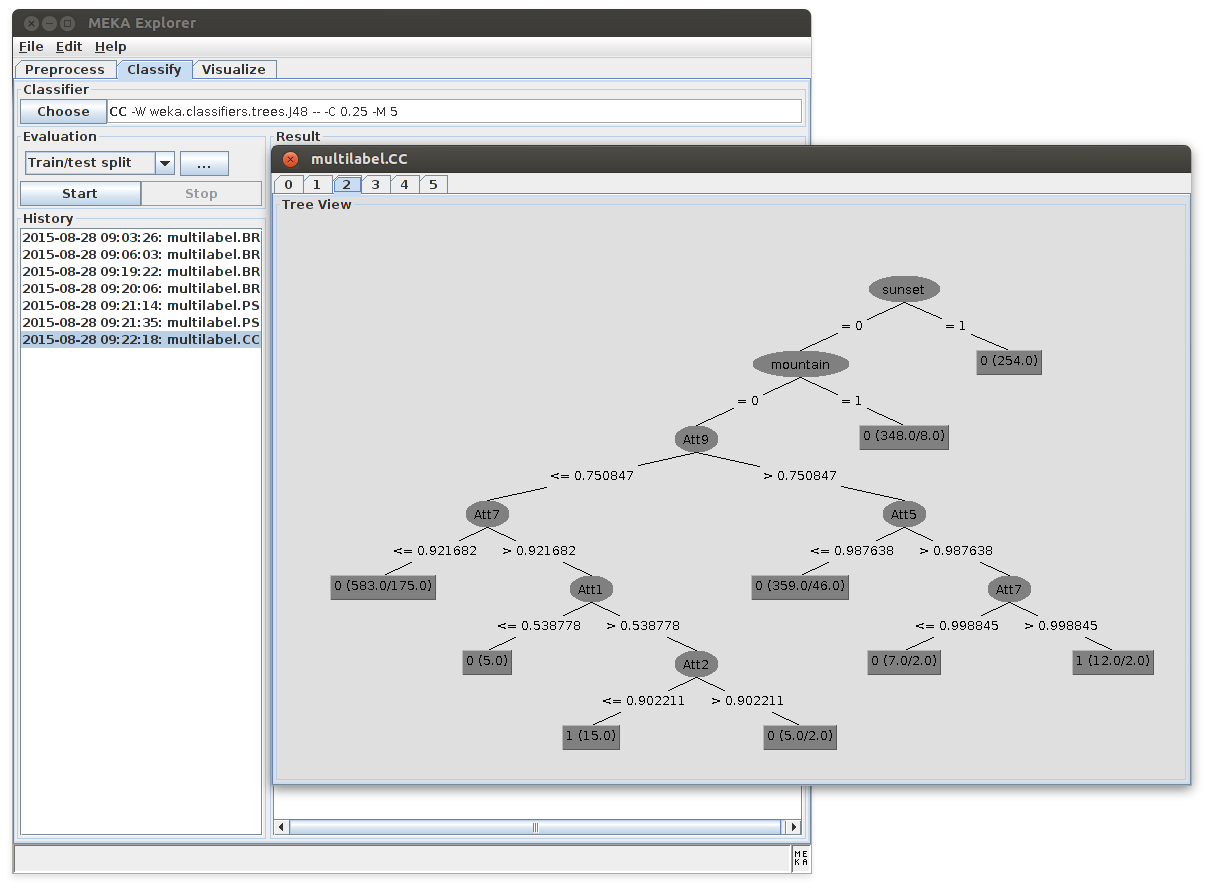
\includegraphics[height=0.75\textwidth]{GUI05.png}
	\caption{\label{screen:graphs} \framework{MEKA}'s GUI interface; viewing a Decision Tree model of \texttt{CC}.}
\end{figure}

\subsection{Examples} 
\label{sec:examples}

In the following we give some examples, with an emphasis on general usage and parameters. An extensive list of examples is given at \url{http://meka.sourceforge.net/methods.html}. 

%\paragraph{Multi-label}

%The methods used in the following examples are detailed in papers papers detailing these methods are available here.

\paragraph{Binary Relevance} (BR) On the \textit{Music} data, loading from two separate sets, using Naive Bayes as a base classifier, calibrating a separate threshold automatically for each label: 
\begin{lstlisting}
java meka.classifiers.multilabel.BR \
  -t data/Music_train.arff \
  -T data/Music_test.arff \
  -threshold PCutL \
  -W weka.classifiers.bayes.NaiveBayes
\end{lstlisting}

\paragraph{Ensembles of Pruned Sets} (EPS; see \cite{EPS}) With 10 ensemble members (the default) on the \textit{Enron} dataset with Support Vector Machines as the base classifier; each \texttt{PS} model is set with \texttt{N=1} and \texttt{P} to a random selection of \texttt{\{1,2,3,4,5\}}:

\begin{lstlisting}
java meka.classifiers.multilabel.meta.EnsembleML \
  -t data/Yeast.arff \
  -W meka.classifiers.multilabel.PS -- \
    -P 1-5 -N 1 -W weka.classifiers.functions.SMO
\end{lstlisting}

\paragraph{Ensembles of Classifier Chains} (ECC; see \cite{ECC2}) With 50 ensemble members (\texttt{-I 50}), and some textual output (\texttt{-output-debug-info}) on the \textit{Enron} dataset with Support Vector Machines as a base classifier:
\begin{lstlisting}
java meka.classifiers.multilabel.meta.BaggingML -I 50 -P 100 \
  -t data/Enron.arff  \
  -output-debug-info -W meka.classifiers.multilabel.CC -- \ 
    -W weka.classifiers.functions.SMO
\end{lstlisting}

\paragraph{Mulan Classifier} (\texttt{RAkEL} see \cite{RAKEL}) With parameters \texttt{\texttt{k=3}, \texttt{m=2C}} where \texttt{C} is the number of labels (these options are hardwired; you need to edit \texttt{MULAN.java} to specify new parameter configurations) on the \textit{Scene} dataset with Decision Trees as the base classifier (remember {\texttt{mulan.jar} must be in the classpath}):
\begin{lstlisting}
java meka.classifiers.multilabel.MULAN -t data/Scene.arff -verbosity 5 \ 
  -S RAkEL2 -W weka.classifiers.trees.J48
\end{lstlisting}
the \texttt{-verbosity 5} options increases the amount of evaluation output.

%\paragraph{Cross Validation} the following carries out cross validation on ECC using Logistic Regression as a base classifier, on the \textit{Music} data.

%\begin{lstlisting}
%java meka.classifiers.multilabel.meta.BaggingML \
%  -x 10 -R -t data/Music.arff \
%  -I 10 -W meka.classifiers.multilabel.CC -- \
%  -W weka.classifiers.functions.Logistic
%\end{lstlisting}

\paragraph{Incremental Classification: Ensembles of Binary Relevance} (see \cite{ECC2,MEDS2}) With 10 ensemble members (default) on the \textit{Enron} dataset with \texttt{NaiveBayesUpdateable} as a base classifier; prequential evaluation taking 20 samples of performance over time:

\begin{lstlisting}
java meka.classifiers.multilabel.incremental.meta.BaggingMLUpdateable\
  -x 20 -t data/Enron.arff \
  -W meka.classifiers.multilabel.incremental.BRUpdateable -- \
    -W weka.classifiers.bayes.NaiveBayesUpdateable
\end{lstlisting}

Under \emph{prequential evaluation}, the cumulative \emph{final} evaluation is reported, and $\texttt{x}$ samples are stored along the way (these can be visualised as a plot over time from within the GUI). An initial window is used for initial training but is not included in evaluation, the equivalent to $1/(\texttt{x}+1)$-th of the data; the remaining data is divided into $\texttt{x}$ windows. If using \emph{batch-incremental evaluation}, evaluation is carried out in batches, but this is non-cumulative (the result is reset before each new batch). This mode is selected with \texttt{-b} on the command line. The \texttt{-x} option is, in this case, considered as the number of batches (minus an original batch used only for training -- similarly to under the prequential option).

\paragraph{Multi-target: Ensembles of Class Relevance} (see \cite{UPM}) The multi-target version of the Binary Relevance classifier) on the \textit{solar flare} dataset with Logistic Regression as a base classifier under $10$-fold cross-validation:
\begin{lstlisting}
java meka.classifiers.multitarget.meta.BaggingMT -x 10 -R \
  -t data/solar_flare.arff \
  -W meka.classifiers.multitarget.CR -- \
    -W weka.classifiers.functions.Logistic
\end{lstlisting}
 
\paragraph{Semi-supervised: EM} with CC with Logistic Regression as a base classifier, using a separate set of unlabelled data (in two separate commands):
\begin{lstlisting}
java meka.classifiers.multilabel.meta.EM -t data-train.arff \
  -T data-unlabelled.arff -d em.saved
java meka.classifiers.multilabel.meta.EM -t data-train.arff \
  -T data-test.arff -l em.saved
\end{lstlisting}
%\begin{lstlisting}
%java -cp meka.jar:weka.jar weka.classifiers.multitarget.meta.BaggingMT -x 5 -R -t data/solar_flare.arff -W weka.%classifiers.multitarget.C    C -- -W weka.classifiers.functions.Logistic
%\end{lstlisting}

{\green Note that the training set is required again in the second command because when \texttt{PCutL} is used (currently the default) it is necessary to know the label cardinality of the training data in order to calibrate a threshold.}

\section{Development}
\label{development}
The following sections explain a bit more in detail of how to obtain MEKA's source code, how to compile it and how to develop new algorithms.

\subsection{Source code}
\label{sourcecode}
For obtaining the source code of MEKA, you have two options:
\begin{itemize}
  \item Using subversion\footnote{\url{http://subversion.apache.org/}}
  \item Release archive
\end{itemize}

\noindent In the case of \textit{subversion}, you can obtain the source code using the following command in the console (or \textit{command prompt} for Windows users):
\begin{lstlisting}
svn checkout svn://svn.code.sf.net/p/meka/code/trunk meka
\end{lstlisting}
This will create a new directory called \texttt{meka} in the current directory, containing the source code and build scripts.

Instead of using subversion, you can simply use the source code that is part of each MEKA release, contained in the \texttt{meka-src-\version.jar} Java archive\footnote{\url{http://en.wikipedia.org/wiki/JAR\_(file\_format)}}. A Java archive can be opened with any archive manager that can handle ZIP files.

\subsection{Compiling}
\label{compiling}
\heading{Using \texttt{Maven}}
\framework{\MEKA} uses \textit{Apache Maven}\footnote{\url{http://maven.apache.org/}} as build tool. You can compile \framework{\MEKA} as follows:
\begin{lstlisting}
mvn clean install
\end{lstlisting}
If you want to generate an archive containing all source code, pdfs and binary jars, then you can use the following commands
(make sure that the version in the \texttt{release.xml} file matches the one in the \texttt{pom.xml}):
\begin{lstlisting}
mvn clean install
mvn -f release.xml package
\end{lstlisting}
Please note, if you develop new algorithms, you should also create a unit test for it, to ensure that it is working properly. See section \ref{unittests} for more details.

\heading{Using IntelliJ IDEA}
After obtaining the source code, you can simply import Meka as a Maven project.
Select \textsf{File $\rightarrow$ New $\rightarrow$ Project from Existing Sources} from the main menu and point to
the directory containing the \texttt{pom.xml} file.

\heading{Using Eclipse}
If you are using the \textit{Eclipse IDE for Java Developers}, then you can import as a Maven project.
Select \textsf{File $\rightarrow$ Import...} and then select {Maven $\rightarrow$ Existing Maven Projects}.
After selecting the root directory with \framework{\MEKA}'s \texttt{pom.xml}, click on \textsf{Finish}.

\subsection{Unit tests}
\label{unittests}
\framework{\MEKA} uses the JUnit 3.8.x unit testing framework.

\noindent A classifier test case is derived from the following abstract super class:
\begin{lstlisting}
meka.classifiers.AbstractMekaClassifierTest
\end{lstlisting}

\noindent A filter test case is derived from the following abstract super class:
\begin{lstlisting}
meka.filters.AbstractMekaFilterTest
\end{lstlisting}

\noindent You can execute all the unit tests by calling the following class from the command-line:
\begin{lstlisting}
mvn test
\end{lstlisting}

\subsection{\label{sec:extending}Extending \framework{\MEKA}}%: Writing New Classifiers

\framework{\MEKA} classifiers are regular \framework{\WEKA} classifiers that extend either the \texttt{MultilabelClassifier} or \texttt{MultiTargetClassifier} class (most of them are \texttt{ProblemTransformationMethod}s), and expect the \texttt{classIndex()} of \texttt{Instance}s and \texttt{Instances}s to indicate the number of target attributes (indexed at the beginning) rather than the class index (see Section \ref{sec:format}). 

The following is an example of a functioning (but extremely minimalistic) classifier, \texttt{TestClassifier}, that predicts $0$-relevance for all labels:

{\small
\lstset{basicstyle=\small\ttfamily,breaklines=true,language=java,frame=L,xleftmargin=\parindent}
\begin{lstlisting}
package meka.classifiers.multilabel;
import weka.core.*;

public class TestClassifier extends ProblemTransformationMethod {
	
    public void buildClassifier(Instances D) throws Exception {
        testCapabilities(D);
        int C = D.classIndex();
    }
    
    public double[] distributionForInstance(Instance x) throws Exception {
        int C = x.classIndex();
       	return new double[C];
    }
    
    public static void main(String args[]) {
        MultilabelClassifier.runClassifier(new TestClassifier(),args);
    }
}
\end{lstlisting}
}

This shows how easy it is to create a new classifier. If it is not a \textit{problem transformation method},
then use the appropriate \framework{\WEKA} superclass and implement the \texttt{MultiLabelClassifier}
interface (\texttt{ProblemTransformationMethod} implements this interface).
For more useful examples see the source code of existing \framework{\MEKA} classifiers.
The \texttt{testCapabilities(D)} line is optional but highly recommended. Note that the \texttt{distributionForInstance}
method returns a \texttt{double[]} array exactly like in \framework{\WEKA}. However, whereas in \framework{\WEKA},
there is one value in the array for each possible value of the single target attribute, in \framework{\MEKA} this
function returns an array of $C$ values, where $C$ is the \emph{number} of target attributes, and the $j$th value of
the array is the \emph{value} corresponding to the $j$th target attribute.

\subsubsection{Building Classifiers}

In the \texttt{buildClassifier(Instances)} method, you build your classifier. Here is where you can take advantage of all of \framework{\WEKA}'s libraries. You can use any \framework{\WEKA} classifier to your needs. The \texttt{m\_Classifier} variable is already available for this, which \textit{already contains} the \framework{\WEKA} classifier you specify on the command line. You can simply do:
{
\lstset{basicstyle=\small\ttfamily,breaklines=true,language=java,frame=L,xleftmargin=\parindent}
\begin{lstlisting}
    public void buildClassifier(Instances D) throws Exception {
        testCapabilities(D);
        int C = D.classIndex();
        D.setClassIndex(0);
        m_Classifier.buildClassifier(D);
    }
\end{lstlisting}
}
to train a classifier to learn the first label of your data (using the other labels, and all other input-space feature attributes). So if you then run on the command line
{
\lstset{basicstyle=\small\ttfamily,breaklines=true,language=java,frame=L,xleftmargin=\parindent}
\begin{lstlisting}
java meka.classifiers.multilabel.TestClassifier -t data/Music.arff \
	-W weka.classifiers.functions.SMO
\end{lstlisting}
}
an instantiation of \texttt{SMO} will already be be available in \texttt{m\_Classifier}. You can also do this explicitly with
{
\lstset{basicstyle=\small\ttfamily,breaklines=true,language=java,frame=L,xleftmargin=\parindent}
\begin{lstlisting}
...
    m_Classifier = new SMO();
    m_Classifier.buildClassifier(D);
...
\end{lstlisting}
}

\subsubsection{Classifying New Instances}

In the multi-label case, for a test \texttt{Instance x}, the \texttt{double[]} array returned by the method \texttt{distributionForInstance(x)} might contain the $0/1$ label relevances, for example (assuming \texttt{-C 5}):
\begin{lstlisting}
	[0.0, 0.0, 1.0, 1.0, 0.0]
\end{lstlisting} 
or it might contain posterior probabilities / prediction confidences / votes for each label, for example:
\begin{lstlisting}
	[0.1, 0.0, 0.9, 0.9, 0.2]
\end{lstlisting} 
where clearly the third and fourth labels are most relevant. Under a threshold of $0.5$ the final classification for \texttt{x} would be \texttt{[0,0,1,1,0]}. \framework{\MEKA} will by default automatically calibrate a threshold to convert all values into $0/1$ relevances like these (see Section \ref{sec:evaluation}). 

%\subsubsection{Multi-target Classifiers}

In the multi-target case, the \texttt{double[]} values returned by the method \texttt{distributionForInstance} must indicate the \emph{relevant value}; for example (assuming \texttt{-C 3}): 
\begin{lstlisting}
	[3.0, 1.0, 0.0]
\end{lstlisting} 
If this were the dataset exemplified in \Sec{sec:format}, this classification would be \texttt{C,1,1} for the class attributes \texttt{category,label,rank}, respectively.

Therefore, at the current release, thresholds are not automatically calibrated for multi-target data. 

Associated probabilistic/confidence may be stored in an extended part of the array, e.g., $\texttt{[C+1,\ldots,2C]}$, for example (if \texttt{-C 6}):
\begin{lstlisting}
	[3.0, 1.0, 0.0, 0.5, 0.9, 0.9]
\end{lstlisting} 
where the $3$-rd \emph{value} is predicted for the first \emph{target variable}, with confidence $0.5$, and so on. Note, however, that this mechanism will be replaced in future versions of \framework{\MEKA}.

\subsubsection{Incremental Classifiers}

\framework{\MEKA} comes with incremental versions of many classifiers as well as incremental evaluation methods, located in the \texttt{meka/classifiers/multilabel/incremental/} folder. Incremental classifiers implement \framework{\WEKA}'s \texttt{UpdatebleClassifier} interface and therefore must implement the \texttt{updateClassifier(Instance)} method. The following extends \texttt{TestClassifier} for incremental learning.

{
\small
\lstset{basicstyle=\small\ttfamily,breaklines=true,language=java,frame=L,xleftmargin=\parindent}
\begin{lstlisting}
package meka.classifiers.multilabel.incremental;
import meka.classifiers.multilabel.TestClassifier;
import weka.classifiers.UpdateableClassifier;
import weka.core.*;

public class TestClassifierUpdateable extends TestClassifier 
    implements UpdateableClassifier{
	
    public void updateClassifier(Instance x) throws Exception {
        int L = x.classIndex();
    }
    
    public static void main(String args[]) {
        IncrementalEvaluation.runExperiment(
            new TestClassifierUpdateable(),args);
    }
}
\end{lstlisting}
}

Note that the \texttt{IncrementalEvaluation} class is called for evaluation in this case; see Section \ref{sec:evaluation}, and example in \Sec{sec:examples}. Note also the \framework{\MOA} framework \cite{MOA} contains more possibilities than \framework{\WEKA}, and its classifiers can be used via \framework{WEKA}'s \texttt{MOA} meta classifier (wrapper), e.g., 
\begin{lstlisting}
java meka.classifiers.multilabel.BRUpdateable -t data/Music.arff \
	-W weka.classifiers.meta.MOA -- -B moa.classifiers.trees.HoeffdingTree
\end{lstlisting}

Note that \framework{\MOA} now also supports \framework{\MEKA} classifiers via a wrapper class.

\subsubsection{Semi-supervised Classifiers}

Semi-supervised classifiers implement \texttt{SemisupervisedClassifier} interface and must implement the method \texttt{setUnlabelledData(Instances)} which is called automatically by the \texttt{Evaluation} class prior to \texttt{buildClassifier(Instances)}. It is up to the classifier to decide what to do with the unlabelled instances. Currently, \framework{\MEKA} assumes that unlabelled instances are the test instances (e.g., supplied with the \texttt{-T} flag). It sets all labels to missing beforehand just in case. In the case of a separate set of unlabelled instances, a model can be built, given unlabelled instances with \texttt{-T}, and then saved/dumped into a file with the \texttt{-d <filename>} option, and loaded again (with the \texttt{-l} option) along with a \emph{different} set with \texttt{-T}.  See the example in \Sec{sec:examples}.

\subsection{Miscellaneous}

Note that \framework{\MEKA}'s home directory is OS-specific,

\begin{itemize}
	\item In Microsoft Windows: \texttt{\%USERPROFILE\%\\mekafiles}
	\item In Unix-based systems: \texttt{\$HOME/.meka}
\end{itemize}

Note that the \texttt{.props} files have preference the following order: 
\begin{enumerate}
	\item the \texttt{jar}
	\item user's home directory
	\item \framework{\MEKA}'s home directory
	\item current directory
\end{enumerate}

\section{Getting Help / Reporting Bugs / Contributing}

A list of methods available using \framework{\MEKA} is maintained at \url{http://meka.sourceforge.net/methods.html} with descriptions and command-line examples.

If you need help with \framework{\MEKA}, you can post your problem on \MEKA's \textsf{Mailing List}: \url{http://sourceforge.net/p/meka/mailman/}.

If you have found a bug with \framework{\MEKA}, you can report in via the \textsf{Tracker}  of \framework{\MEKA}'s \url{SourceForge.net} site: \url{http://sourceforge.net/p/meka/bugs/}.

If you would like to contribute to \framework{\MEKA}, such as adding new classifiers, please get in touch with the developers.

More information (such as contact information) can be found at the \framework{\MEKA} website: \url{http://meka.sourceforge.net}.

\begin{thebibliography}{10}

\bibitem{MOA}
Albert Bifet, Geoff Holmes, Richard Kirkby, and Bernhard Pfahringer.
\newblock Moa massive online analysis, 2010.
\newblock \url{http://mloss.org/software/view/258/}.

\bibitem{WEKA}
Mark Hall, Eibe Frank, Geoffrey Holmes, Bernhard Pfahringer, Reutemann Peter,
  and Ian~H. Witten.
\newblock The weka data mining software: An update.
\newblock {\em SIGKDD Explorations}, 11(1), 2009.

\bibitem{Thesis}
Jesse Read.
\newblock {\em Scalable Multi-label Classification}.
\newblock PhD thesis, University of Waikato, 2010.

\bibitem{MEDS2}
Jesse Read, Albert Bifet, Bernhard Pfahringer, and Geoffrey Holmes.
\newblock Scalable and efficient multi-label classification for evolving data
  streams.
\newblock {\em Machine Learning}, 2012.
\newblock Accepted for publication.

\bibitem{EPS}
Jesse Read, Bernhard Pfahringer, and Geoff Holmes.
\newblock Multi-label classification using ensembles of pruned sets.
\newblock In {\em ICDM'08: Eighth IEEE International Conference on Data
  Mining}, pages 995--1000. IEEE, 2008.

\bibitem{ECC2}
Jesse Read, Bernhard Pfahringer, Geoffrey Holmes, and Eibe Frank.
\newblock Classifier chains for multi-label classification.
\newblock {\em Machine Learning}, 85(3):333--359, 2011.

\bibitem{MMD}
G.~Tsoumakas, I.~Katakis, and I.~Vlahavas.
\newblock Mining multi-label data.
\newblock In O.~Maimon and L.~Rokach, editors, {\em Data Mining and Knowledge
  Discovery Handbook}. 2nd edition, Springer, 2010.

\bibitem{RAKEL}
Grigorios Tsoumakas and Ioannis~P. Vlahavas.
\newblock Random k-labelsets: An ensemble method for multilabel classification.
\newblock In {\em ECML '07: 18th European Conference on Machine Learning},
  pages 406--417. Springer, 2007.

\bibitem{UPM}
Julio~H. Zaragoza, Luis~Enrique Sucar, Eduardo~F. Morales, Concha Bielza, and
  Pedro Larra{\~n}aga.
\newblock Bayesian chain classifiers for multidimensional classification.
\newblock In {\em 24th International Conference on Artificial Intelligence
  (IJCAI '11)}, pages 2192--2197, 2011.

\bibitem{MT}
Bernard Zenko and Saso Dzeroski.
\newblock Learning classification rules for multiple target attributes.
\newblock In {\em PAKDD '08: Twelfth Pacific-Asia Conference on Knowledge
  Discovery and Data Mining}, pages 454--465, 2008.

\end{thebibliography}


\end{document}
